% Chapter Template

\chapter{Instrumentation} % Main chapter title

\label{ChapterInstrumentation} 

%----------------------------------------------------------------------------------------

%----------------------------------------------------------------------------------------

\section{Ulysses}
\label{sec:ulysses}
The Ulysses spacecraft \citep{wenzel_ulysses} was launched in 1990 and orbited the sun for nearly 20 years as a joint ESA/NASA project.
Ulysses' most remarkable feature is its out-of-ecliptic orbit with an maximum heliographic latitude of $80.1\,^\circ$.
As the first spacecraft it was hence capable of taking in situ measurements from above the poles of the sun.
\\ \\
Thus, the primary goal of the mission was to study the heliosphere in three dimensions. In detail some of the original main objectives were:
\begin{itemize}
	\item to study the interplanetary magnetic field and the solar wind, especially its composition, the origin and waves and shocks within the solar wind plasma
	\item to investigate galactic cosmic rays and energetic particles
	\item to improve the knowledge about interplanetary dust
	\item to explore the neutral component of interstellar gas
\end{itemize}
Some secondary objectives included e.g. the investigation of Jupiter's magnetosphere during the Jupiter flyby and the search for gravitational waves and for gamma-ray burst sources \citep{wenzel_ulysses}.
\\
For these aims Ulysses was equipped with a wide range of different instruments and antennas. One of the in situ instruments is the Solar Wind Ion Composition Spectrometer, that will be described in the next chapter.
\begin{figure}[h]
	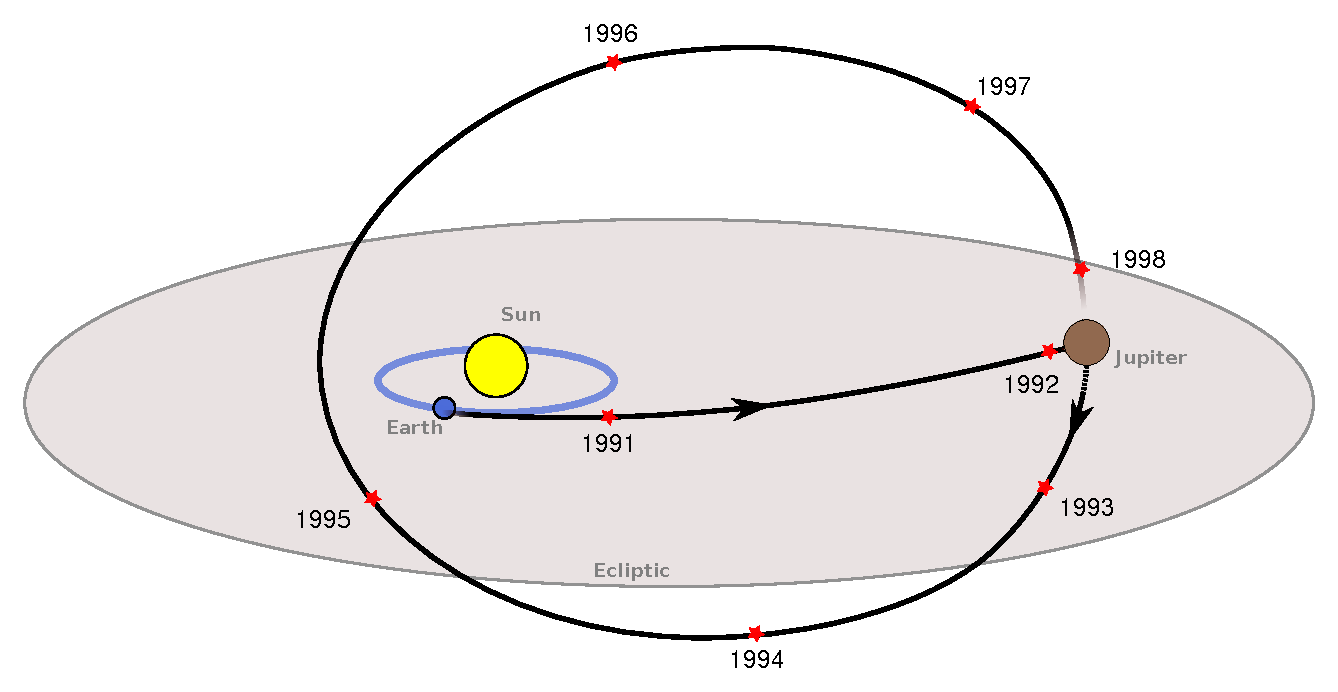
\includegraphics[width=0.8\textwidth]{Figures/ulysses_trajectory.pdf}
	\centering
	\caption{A sketch of Ulysses' first orbit. After the launch from earth in 1990 the spacecraft was sent to Jupiter from where it left the ecliptic on an elliptical orbit around the sun with perihelion at $1.3\,\mathrm{AU}$ and aphelion at $5.4\,\mathrm{AU}$. Due to the orbit's high latitude of $\sim 80 \, ^\circ$ Ulysses crosses the Sun's pole regions two times between 1994 and 1996. Figure after \citet{esa_orbit}.}
	\label{fig:trajectory}
\end{figure}
\\ \\
A sketch of Ulysses unique orbit is shown in figure \ref{fig:trajectory}.
Ulysses was launched in October 1990 and left earth's gravitational field with $15.4\,\mathrm{km/s}$. Starting with a flyby maneuver around Jupiter Ulysses was sent onto its highly elliptical orbit.
With an orbital period of 6.2 years Ulysses completed nearly three orbits around the sun until communication was shut down in June 2009 due to the expiring of the radioisotope thermal generators.
Within the mission's long lifetime the Sun's behaviour over its activity cycle of 22 years could be studied. 
\\ \\
eccentricity, elliptical orbit...
\\ \\
aspect angle (antenna)-- Power: RHU because too far away for solar panels (and radiation belt of Jupiter) -- rotation stabilization --  mission was extended multiple times
\\ \\
Abbildung Sun Cycles?
\\ \\ 
spinstabilisiert, Antenna fast Rotationsachse, Antenne zeigt zur Erde, woher Daten (Ulysses, SWICS, Erde)
\\ \\
Rotation: Spi und 1 EpQ pro Spin
\\ \\ 
Importance PUIs: ref to PUI-Kapitel und zu objectives
%
%
%
%
%
\section{SWICS}

\subsection{Introduction and Objectives}
The Solar Wind Ion Composition Spectrometer (SWICS, \citet{gloeckler_1992}) is a time-of-flight mass spectrometer mounted on the spacecraft Ulysses (s. section \ref{sec:ulysses}). The instrument is designed to determine the elemental and charge-state composition and the velocity distribution of solar wind ions. With an energy-per-charge range from $0.16 \, \mathrm{keV/e}$ to $59.6 \, \mathrm{keV / e}$ SWICS is in principle able to measure every solar wind ion species from protons to iron with any typical charge state. Depending on the individual ion, energies from $E < 1 \,\mathrm{keV}$ up to $E > 1 \, \mathrm{MeV}$ are covered.
\\ \\
Additionally, the flight spare of SWICS has been mounted on the spacecraft ACE (TODO: ref Stone 1998)
\\ \\ 
Also capable of measuring PUIs! Erstmals gesehen...?
\\ \\
SWICS measures the mass $m$, the charge $q$ and the energy $E_{SSD}$ of entering ions by a combination of three separate measurements: The \textit{electrostatic deflection analyzer} within SWICS entrance systems is used for determining the energy per charge of a particle. Within the time-of-flight/energy section the particle's time-of-flight ($ToF$) and energy ($E_{SSD}$) are measured. \\ 
Todo: Bild von SWICS, neben den beiden sieht man noch die Elektronik...
\\ \\
mounted on the sun-facing side of Ulysses
\\ \\
Opening angles: $\pm\, 2$ deg perp, $90$ deg parallel  
\\ \\
Richtungsauflösung Detektoren
\\ \\ 
In the following section the measurement is described in more detail.
\subsection{Principle of Measurement / Identification of Particles}
\begin{figure}[h]
	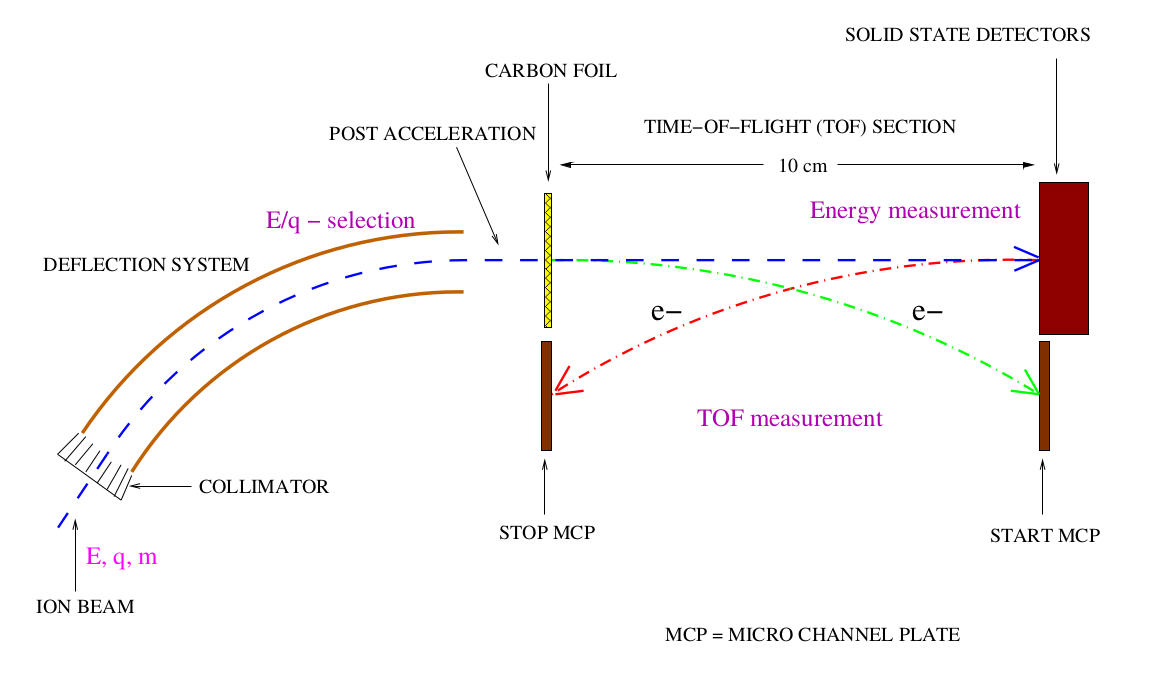
\includegraphics[width=0.8\textwidth]{Figures/Lars_Swics.png}
	\centering
	\caption{test}
	\label{fig:lars_swics}
\end{figure}


\begin{figure}[h]
	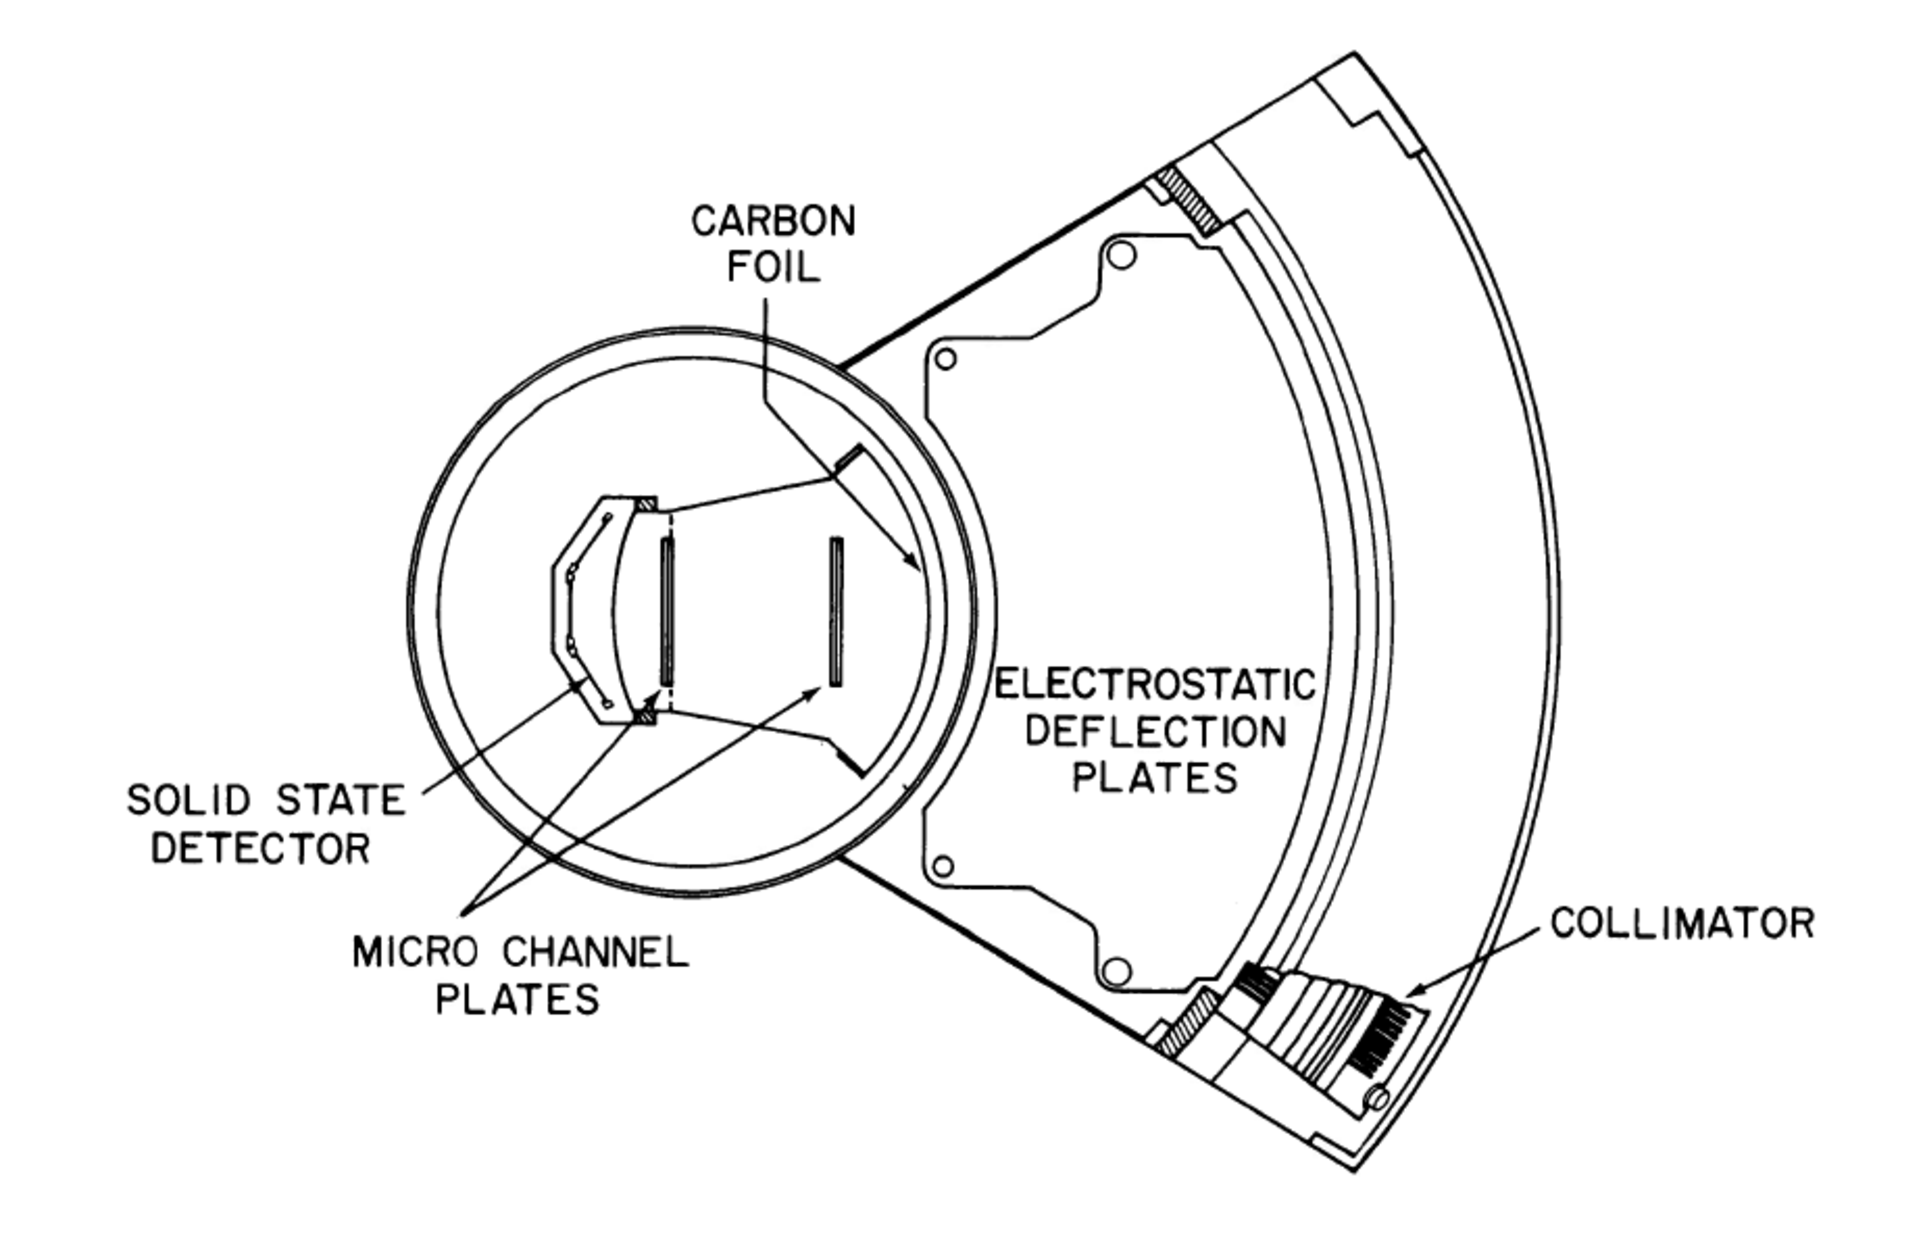
\includegraphics[width=0.8\textwidth]{Figures/swics_sensor.pdf}
	\centering
	\caption{test}
	\label{fig:sensor_swics}
\end{figure}
\subsubsection{Collimator and Electrostatic Analyzer}
\label{sec:EpQ}
Particles enter the instrument through the entrance collimator. It restricts particles to the ones with a trajectory that is parallel to the collimator slits. The geometry of the collimator is curved "fan-shaped"...TODO: Kollimatorgeometrie beschreiben \\
Within the TODO: Two sections
After the collimator particles have to pass the electrostatic analyzer. It is split up into two sections -- energies from $0.16$ to $14\,\mathrm{keV/e}$ are covered by the proton/helium channel. Particles within this range of energy will be filtered by their EpQ and after an post-acceleration will be counted by a solid-state detector. 
As this simple measurement principle is very limiting for our analysis we will focus on the main channel that is suitable for a full $m$-vs.-$mpq$ analysis.
The main channel covers an EpQ range of $0.65$ to $60\,\mathrm{keV/e}$. A particle can only pass through the pair of curved deflection plates if its kinetic energy per charge equals a certain ratio that is given by the voltage between the two plates. To measure particles of different EpQ the deflection voltage is stepped through 64 logarithmically spaced values from TODO to TODO. As the voltage steps once per spin of Ulysses (every 12 seconds), a complete voltage cycle lasts $\sim$ 12.8 minutes. 
Every step has a relative uncertainty of $\Delta E/q \approx 5\%$ that is due to the finite space between the plates. TODO: Plot
  
\subsubsection{Time-of-flight measurement}
After passing the electrostatic analyzer ions are post-accelerated by an constant potential drop of ~$30\,\mathrm{kV}$. They enter the ToF chamber with penetrating through a thin ($\sim 3\,\mu \mathrm{g / cm^2}$) carbon foil where secondary electrons are emitted. These electrons are guided to a microchannel plate detector where a start signal is triggered. The stop signal is triggered after the particles have traversed a distance of $10\,\mathrm{cm}$ and hit one of the solid state detectors, where secondary electrons are emitted again. By combining the time stamps of the start and the stop signal the particle's ToF has been measured.
\subsubsection{Energy measurement}
Furthermore, the particle's energy is measured when they hit one of the three solid state detectors (SSD). The detectors have each an active area of $1.5 x 1.3 \,\mathrm{cm^2}$ and their orientation of the detectors can be seen in TODO. While the central detector is aligned perpendicular to the symmetry axis of SWICS, the other two detectors are slightly tilted with respect to this axis. Particles with different angles of incidence along the width of the collimator can be detected this way.
\\ \\
Thus, a wide field-of-view is provided, allowing measurements of particles, die schief reinkommen. Das passt zur Begrenzung vom Kollimator. Man kann auch unterscheiden, welcher getroffen wurde.\\
Verfälschungen? Folie etc? \\ 
The measured energy $E_{SSD}$ is often referred to as \textit{residual energy} in literature. This is potentially misleading as the particles might have more energy due to the post-acceleration 
%%%
\\ \\ \\
One of SWICS' main objectives is the measurement of the composition of incident particles. An ion and its charge state can be fully identified with the knowledge of its mass $m$ and its mass-per-charge $mpq$. 
With the measurement of the ToF, the energy $E_{SSD}$ and the knowledge of the EpQ-step we can calculate the mass, mpq and velocity of an ion $i$ with the following set of equations:
\begin{align}
m_i &= 2\,E_{SSD} \left( \frac{Tof}{d}\right)^2 \label{eq:swics_set1}\\
\frac{m_i}{q_i} &= 2 \left(EpQ + V_{PAC}\right) * \left(\frac{Tof}{d}\right)^2 \label{eq:swics_set2} \\
v_i &= \sqrt{2\,EpQ\,\frac{q_i}{m_i}},
\label{eq:swics_set3}
\end{align}
where $d$ is the length of the time-of-flight section and $V_{PAC}$ is the post-acceleration voltage. $v$ denotes the ion's initial velocity when entering the instrument and is not to be confused with its velocity during the time-of-flight measurement, that is altered particularly by the post-acceleration.
\\ \\ \\HISCALE: "The experiment provides information about the spatial origin of events by treating each spin as eight sectors of approximately equal duration."